% Provenance (never printed): sources/book2/BRIEFS.md, g10-05. Market supply, the law of supply,
% shifts, short-run and long-run supply. Real numbers: figdata/grade-10/05-supply/ (EIA crude oil,
% BLS gasoline price and CPI-U, FAOSTAT soya area). Brenland and Kestria numbers are invented.
\chapter{Supply}\label{ch:g10:supply}

In 2008 the United States produced about 5.0 million barrels of crude oil a day, little more than half of what it had
produced in 1985, and its old fields were running dry. Then the price
of oil stayed high for years: at the pump, a gallon of gasoline cost between \usd{4.01} and \usd{4.98} in today's
money every year from 2010 to 2014. Firms that had been testing new ways to reach oil locked in thin layers of rock
--- drilling sideways for kilometres and cracking the rock open with water under pressure --- now found it paid to
use them on a large scale. By 2014 American production had reached 8.8 million barrels a day; by 2024, 13.3 million,
more than in any year since the series began in 1976.
% figdata: crude_us (1985 8.97; 2008 5.00; 2010-2014 price 4.01-4.98; 2014 8.79; 2024 13.27)

The opening chart shows the two series. The quantity offered responded to the price, but not at once: the first
years of high prices brought little, and the big response came later. This chapter builds the supply side of a
market, and the role of time in it.

\begin{openingchart}{Crude oil production in the United States, in millions of barrels a day (top), and the price of
regular gasoline, in 2024 dollars per gallon (bottom), 1976--2024. The price at the pump follows the price of crude oil.}{US Energy Information Administration, international energy statistics; US Bureau of Labor
Statistics, average retail prices and CPI-U all items}
\begin{tikzpicture}
\begin{groupplot}[group style={group size=1 by 2, vertical sep=0.9cm, x descriptions at=edge bottom},
  omtime, width=0.88\linewidth, height=4.6cm, xmin=1975, xmax=2025, xtick={1980,1985,...,2020}]
\nextgroupplot[width=0.88\linewidth, ymin=4, ymax=14, ylabel={million barrels a day}]
\addplot[omDef, thick, mark=*, mark size=0.8pt] table[x=year, y=mbd] {figdata/grade-10/05-supply/out/crude_us.csv};
\nextgroupplot[width=0.88\linewidth, ymin=1.5, ymax=5.5, ylabel={dollars per gallon}]
\addplot[omThm, thick, mark=*, mark size=0.8pt] table[x=year, y=price] {figdata/grade-10/05-supply/out/crude_us.csv};
\end{groupplot}
\end{tikzpicture}
\end{openingchart}

\begin{recall}
From the grades 6--9 volume: the \emph{quantity supplied} is the amount sellers offer at a given price; a \emph{supply
table} and a \emph{supply curve} show it for several prices. A firm's \emph{total cost} is its \emph{fixed cost} plus its
\emph{variable cost}, and its \emph{profit} is revenue minus total cost. From \cref{ch:g10:demand}: the market curve is the
horizontal sum of the individual ones, and a change in anything but the good's own price shifts the curve.
\end{recall}

\section{The quantity offered at each price}\label{sec:g10:supply:offered}

A seller offers a unit for sale when the price covers what that unit costs to produce, including what the seller's time and
money could earn elsewhere. Each extra unit is usually dearer to produce than the one before: the bakery's oven is full,
bakers must work at night and be paid more, flour must be bought from a further mill. So the higher the price, the more
units are worth offering.

Two bakeries in a town of Brenland sell bread at a price $p$ in dalens per loaf (quantities in hundreds of loaves a day).
Bakery A offers $q_A = 2p - 4$ as long as $p \ge 2$, and nothing below 2 dalens, the lowest price at which it bakes at all.
Bakery B, with an older oven, offers $q_B = 3p - 15$ as long as $p \ge 5$.

\begin{definition}[Market supply]\label{def:g10:supply:market-supply}
The \emph{market supply}\index{market supply} of a good gives, at each price, the total quantity that all the sellers in
the market offer: the sum of the individual quantities supplied at that price.
\end{definition}

As for demand, the curves are added horizontally:
\[
  Q^s(p) = \begin{cases} 0 & \text{if } p < 2, \\ 2p - 4 & \text{if } 2 \le p < 5, \\ (2p - 4) + (3p - 15) = 5p - 19 &
  \text{if } p \ge 5 . \end{cases}
\]
At $p = 5$ the first piece gives $10 - 4 = 6$ and the second $25 - 19 = 6$: the \omterm{def:g10:supply:market-supply}{market supply} is continuous, with a kink at
$(6, 5)$ where Bakery B starts baking.

\begin{omfigure}
\begin{tikzpicture}[econ, x=0.34cm, y=0.55cm]
\draw[econ axes] (0,10.5) node[left, font=\small] {price $p$} |- (29,0) node[below left=12pt and 0pt, font=\small] {quantity (hundreds of loaves)};
\draw[supply, omThm!45] (0,2) -- (14,9);
\draw[supply, omThm!45] (0,5) -- (12,9);
\draw[curve] (0,2) -- (6,5) -- (26,9);
\draw[guide] (0,5) -- (6,5) -- (6,0);
\draw[guide] (0,9) -- (26,9) -- (26,0);
\node[eqpoint] at (6,5) {};
\foreach \y in {2,5,9} \draw (0,\y) -- (-0.3,\y) node[left, font=\footnotesize] {\y};
\foreach \x in {6,12,14,26} \draw (\x,0) -- (\x,-0.25) node[below, font=\footnotesize] {\x};
\node[font=\footnotesize, text=omThm!80!black, anchor=west] at (12.5,8) {A};
\node[font=\footnotesize, text=omThm!80!black, anchor=east] at (5,7.6) {B};
\node[font=\footnotesize, anchor=north west] at (16.5,6.6) {market, $5p - 19$};
\end{tikzpicture}

{\small The supplies of Bakery A and Bakery B (light) and the \omterm{def:g10:supply:market-supply}{market supply} (black), added horizontally. Below 5 dalens only
A bakes; above it both do, and the market curve is flatter. At 9 dalens A offers 14, B offers 12 and the market 26.}
\end{omfigure}

\begin{definition}[Law of supply]\label{def:g10:supply:law}
The \emph{law of supply}\index{law of supply} states that, \omterm{def:g10:economic-models:other-things-equal}{other things equal}, the quantity supplied of a good rises when its
price rises: the supply curve slopes upward.
\end{definition}

The \omterm{def:g10:supply:law}{law of supply} is less universal than the \omterm{def:g10:demand:law}{law of demand}. When a firm's cost per unit \emph{falls} as it grows, because it
spreads a large fixed cost over more units, the reasoning above fails; grade 11 deals with such firms. For most markets with
many sellers, and for the time spans of this chapter, the supply curve slopes upward.

\begin{measure}[What a supply curve shows]
Read a supply curve sideways: at a quantity $Q$, its height is the lowest price at which the $Q$-th unit is offered. That price
is the cost of producing that unit for the seller who produces it, the \emph{marginal seller}. At 9 dalens in the figure above,
the 26th hundred loaves is baked because 9 dalens just covers its cost; the first hundred loaves of Bakery A cost much less. A
\omterm{def:g10:supply:market-supply}{market supply} curve is therefore a list of costs, ranked from the cheapest unit to the dearest. It is not a measure of what
the average unit costs, and it is not something a government or a firm writes down: it is the result of many sellers' separate
decisions.
\end{measure}

\section{What moves the curve}\label{sec:g10:supply:shifts}

The supply curve is drawn for a given technology, given input prices and a given number of sellers. When one of them changes,
the quantity offered at every price changes: the curve shifts.

\begin{itemize}
\item \textbf{Input prices.} A rise in the price of flour, energy or labour raises the cost of every loaf: at each price, fewer
  loaves are worth baking, and the curve shifts left (up).
\item \textbf{Technology.} A better oven, a new seed or a new way of drilling lowers costs: the curve shifts right (down).
\item \textbf{The number of sellers.} New firms add terms to the horizontal sum; firms that close remove them.
\item \textbf{Expectations.} A seller who expects a higher price next year may hold back part of this year's output, if it can
  be stored.
\item \textbf{Nature and rules.} A drought shifts the supply of grain left; a rule that limits fishing shifts the supply of fish
  left.
\end{itemize}

\begin{example}[Dearer flour]\label{ex:g10:supply:flour}
The price of flour rises, and each loaf of Bakery A now costs 1 dalen more to bake. Whatever price A needed before for a given
quantity, it now needs 1 dalen more: its supply becomes $q_A = 2(p - 1) - 4 = 2p - 6$, for $p \ge 3$. At a price of 4 dalens, A
offered 4 hundred loaves and now offers 2. The curve has moved up by 1 dalen, which is the same as moving left by 2 hundred
loaves, since A's quantity changes by 2 for each dalen.
\end{example}

\begin{proposition}[A cost rise shifts supply up by the cost]\label{prop:g10:supply:shift}
If a seller's supply is $q = c\,(p - m)$ for $p \ge m$, with $c > 0$, and the cost of every unit rises by $t$ dalens, its new
supply is $q = c\,(p - m - t)$ for $p \ge m + t$. The curve moves up by $t$; at any price, the quantity offered falls by $c\,t$
(or to zero).
\end{proposition}
\begin{proof}
Before the rise, the seller offers its $q$-th unit at the price $m + q/c$, which is the cost of that unit. After the rise each unit
costs $t$ more, so the $q$-th unit is offered at $m + t + q/c$, that is $q = c\,(p - m - t)$. At a given price $p \ge m + t$ the
quantity falls from $c(p - m)$ to $c(p - m) - ct$, a fall of $ct$.
\end{proof}

\section{Time to adjust}\label{sec:g10:supply:time}

A higher price can raise output in two ways. Existing firms can use their equipment more intensively: an extra shift, more
fertiliser, an old well pumped harder. That is quick but limited. Or firms can add capacity: new ovens, new fields, new wells,
new firms entering the market. That is slow, because capacity takes time to plan, finance and build, but it is far larger.

\begin{omfigure}
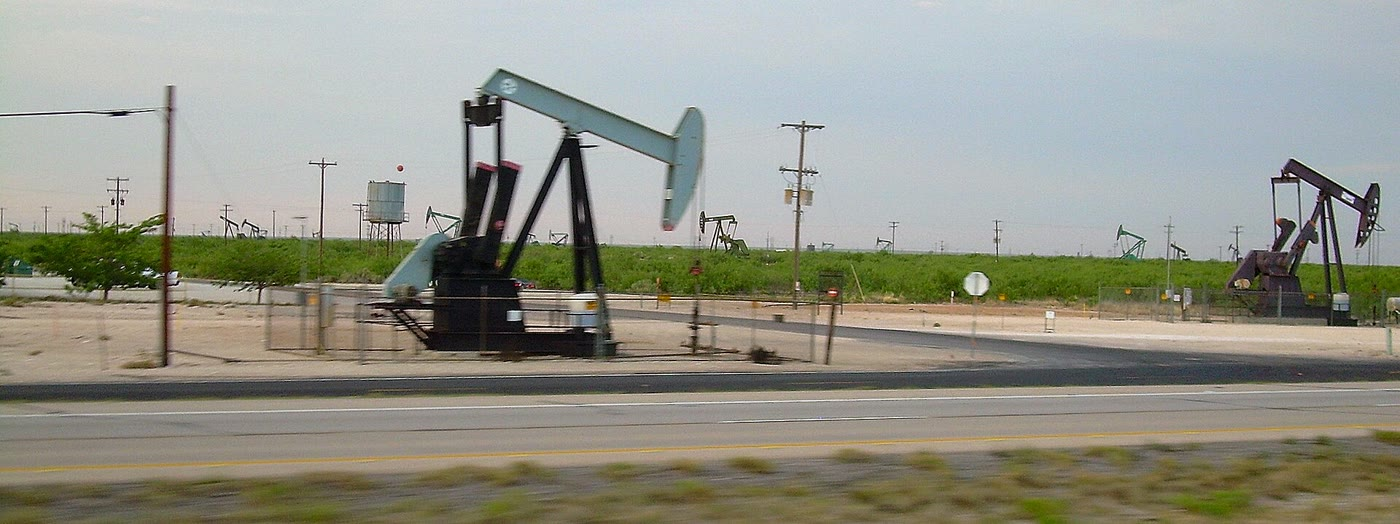
\includegraphics[width=0.58\linewidth]{images/book2/photos/g10-supply-pumpjacks-midland.jpg}

{\small Pumpjacks on oil wells near Midland, Texas, 2006. A well that exists can be pumped harder at once; a new one has to be drilled first.}
\end{omfigure}

\begin{definition}[Short-run and long-run supply]\label{def:g10:supply:short-run}
\emph{Short-run supply}\index{short-run supply} gives the quantity offered at each price when firms can change how much they use
their existing capacity, but not the capacity itself or the number of firms. \emph{Long-run supply}\index{long-run supply} gives
the quantity offered when there has been time for firms to build or close capacity and for firms to enter or leave the market.
\end{definition}
\phantomsection\label{def:g10:supply:long-run}

\begin{example}[Two supply curves through one point]\label{ex:g10:supply:two-curves}
A market sells 500 tonnes a month at 40 dalens. Its \omterm{def:g10:supply:short-run}{short-run supply} is $Q = 300 + 5p$ and its \omterm{def:g10:supply:short-run}{long-run supply} is $Q = -300 + 20p$:
both give 500 at $p = 40$. If the price rises to 50 and stays there, the short-run quantity is $300 + 250 = 550$, 10\,\% more. Over
the following years firms add capacity, and the quantity reaches $-300 + 1000 = 700$, 40\,\% more. The long-run response is four
times the short-run one.
\end{example}

\begin{omfigure}
\begin{tikzpicture}[econ, x=0.017cm, y=0.12cm]
\draw[econ axes] (300,62) node[left, font=\small] {$p$} |- (800,25) node[below left=12pt and 0pt, font=\small] {$Q$ (tonnes)};
\draw[supply] (425,25) -- (600,60);
\draw[supply, shifted] (300,30) -- (900*0.8,51);
\draw[guide] (300,40) -- (500,40) -- (500,25);
\draw[guide] (300,50) -- (700,50) -- (700,25);
\draw[guide] (550,50) -- (550,25);
\node[eqpoint] at (500,40) {}; \node[eqpoint] at (550,50) {}; \node[eqpoint] at (700,50) {};
\foreach \y in {40,50} \draw (300,\y) -- (295,\y) node[left, font=\footnotesize] {\y};
\foreach \x in {500,550,700} \draw (\x,25) -- (\x,24) node[below, font=\footnotesize] {\x};
\node[font=\footnotesize, text=omThm!80!black, anchor=west] at (585,58) {short run, $300 + 5p$};
\node[font=\footnotesize, text=omThm!80!black, anchor=north west] at (640,44) {long run, $-300 + 20p$};
\end{tikzpicture}

{\small \omterm{def:g10:supply:short-run}{Short-run supply} (steep) and \omterm{def:g10:supply:short-run}{long-run supply} (flat, dashed) through the same point, 500 tonnes at 40 dalens. A lasting
rise of the price to 50 brings 550 tonnes at first and 700 once capacity has adjusted.}
\end{omfigure}

\begin{model}{Supply with time to adjust}
\assumes Sellers offer each unit whose cost the price covers; capacity and the number of firms are fixed in the short run and
  adjust, with a delay, when prices stay high or low.
\predicts A lasting price rise raises the quantity supplied a little at first and much more after some years; a lasting fall cuts
  it a little at first, and more as capacity closes.
\tested Consistent with it: US crude oil after 2008, little response in the first years of high prices, then a rise of
  three-quarters by 2014 as new wells were drilled; Brazil's soya area, which quadrupled over three decades as farmland was
  converted. Neither record separates a move along \omterm{def:g10:supply:short-run}{long-run supply} from a shift of it (new drilling methods, tropical seed,
  world demand); a test would need the price and the cost shifts measured together.
\breaks When capacity is fixed by nature or by rule (land by the sea, a number of taxi licences), \omterm{def:g10:supply:short-run}{long-run supply} is no larger than
  \omterm{def:g10:supply:short-run}{short-run supply}; and when technology changes at the same time, as with the new drilling methods, the long-run curve itself moves.
\end{model}
% figdata: crude_us (2008 5.00 -> 2014 8.79: +76 %); soy_area (bra 1990 11.49 -> 2024 45.91: x 4.0)

The opening chart also shows the response running backwards. The price at the pump fell from \usd{4.46} in 2014 to \usd{2.80} in
2016. American crude production fell, but only from 9.45 million barrels a day in 2015 to 8.85 million in 2016: wells already
drilled kept pumping, because once a well exists the cost of pumping one more barrel is small. What stopped was the drilling of new
wells. Then production grew again, to 12.25 million barrels a day in 2019, at prices lower than those of 2011--2014. The cost of the
new methods had fallen as firms learned to use them: the supply curve had moved right.
% figdata: crude_us (2014 price 4.46, 2016 2.80; mbd 2015 9.45, 2016 8.85, 2019 12.25)

\begin{omchart}{Area harvested of soya beans, Brazil and the United States, 1990--2024, in millions of hectares.}{FAOSTAT,
crops and livestock products, area harvested}
\begin{tikzpicture}
\begin{axis}[omtime, width=0.84\linewidth, height=5.6cm, xmin=1989, xmax=2025, ymin=0, ymax=50,
  ylabel={million hectares}, xtick={1990,1995,...,2020}, legend pos=south east]
\addplot[omDef, thick] table[x=year, y=bra] {figdata/grade-10/05-supply/out/soy_area.csv};
\addlegendentry{Brazil}
\addplot[omThm, thick] table[x=year, y=usa] {figdata/grade-10/05-supply/out/soy_area.csv};
\addlegendentry{United States}
\end{axis}
\end{tikzpicture}
\end{omchart}

The second chart shows how slowly capacity can grow. Brazil harvested soya beans on 11.49 million hectares in 1990 and on 45.91 million in
2024, four times as much; the United States, whose good farmland was already in use, went from 22.87 to 34.82 million. Converting
pasture and savanna into soya fields, building roads and storage, and adapting seed to tropical soils took decades. For a crop, the
long run is a generation.
% figdata: soy_area (bra 11.49, 45.91; usa 22.87, 34.82)

\section{Exercises}

\begin{exercise}[$\star$]\label{exo:g10:supply:1}
A dairy offers \num{1000} litres a day at 1 dalen a litre, \num{1400} at 1.2 dalens and \num{1700} at 1.4 dalens. Is this consistent with
the \omterm{def:g10:supply:law}{law of supply}? By how many litres does the quantity offered rise for each tenth of a dalen between 1 and 1.4?
\end{exercise}

\begin{exercise}[$\star$]\label{exo:g10:supply:2}
For the supply of apples, say whether each event shifts the curve left, right, or not at all: (a) a late frost; (b) the price of apples
rises; (c) a cheaper machine for picking; (d) higher wages for farm workers; (e) new orchards planted five years ago start bearing fruit.
\end{exercise}

\begin{exercise}[$\star$]\label{exo:g10:supply:3}
Explain the difference between ``supply rose'' and ``the quantity supplied rose''. Give an example of each for the market for taxis.
\end{exercise}

\begin{exercise}[$\star$]\label{exo:g10:supply:4}
Read the opening chart. In which year was US crude production lowest, and about how large was it? In which later year did it first
pass its 1985 level?
\end{exercise}

\begin{exercise}[$\star$]\label{exo:g10:supply:5}
Two sellers have the supplies $q_1 = p - 2$ (for $p \ge 2$) and $q_2 = 2p - 8$ (for $p \ge 4$). How much does the market offer at a price
of 3, and at a price of 6?
\end{exercise}

\begin{exercise}[$\star\star$]\label{exo:g10:supply:6}
Bakery B's supply is $q_B = 3p - 15$ for $p \ge 5$. A rise in its energy bill adds 2 dalens to the cost of every loaf. Write
its new supply. How much does it offer at 8 dalens, before and after?
\end{exercise}

\begin{exercise}[$\star\star$]\label{exo:g10:supply:7}
A new oven lowers the cost of every loaf at Bakery A by 1.5 dalens. Write A's new supply and the new \omterm{def:g10:supply:market-supply}{market supply} for prices of
5 dalens or more. How much more does the market offer at 9 dalens?
\end{exercise}

\begin{exercise}[$\star\star$]\label{exo:g10:supply:8}
The price of fish rises by 20\,\% and stays there. Predict the response of the quantity of fish offered after a week, after a year, and
after ten years, and explain the difference. What could stop the long-run response?
\end{exercise}

\begin{exercise}[$\star\star$]\label{exo:g10:supply:9}
Read the second chart. By how many million hectares did Brazil's soya area grow between 1990 and 2024, and by how many the United States'?
In which country was the response larger in proportion?
\end{exercise}

\begin{exercise}[$\star\star$]\label{exo:g10:supply:10}
Three sellers have the supplies $q_1 = 2p - 2$ (for $p \ge 1$), $q_2 = p - 3$ (for $p \ge 3$) and $q_3 = 4p - 24$ (for $p \ge 6$). Write the
\omterm{def:g10:supply:market-supply}{market supply}, with its pieces, and give its kinks.
\end{exercise}

\begin{exercise}[$\star\star$]\label{exo:g10:supply:11}
Brenland's furniture makers import all their timber. The government bans timber imports from Kestria, which supplied half of it, and the
price of timber in Brenland rises. Predict the effect on the supply of furniture in Brenland, and on the supply of furniture in Kestria.
\end{exercise}

\begin{exercise}[$\star\star\star$]\label{exo:g10:supply:12}
Describe an observation that would contradict the model of supply with time to adjust. Use the example of a crop whose price rises by half
and stays high for ten years.
\end{exercise}

\begin{exercise}[$\star\star\star$]\label{exo:g10:supply:13}
Using the opening chart, explain why US crude production fell only a little between 2015 and 2016, when the price at the pump fell by more
than a third between 2014 and 2016. Distinguish the cost of pumping from an existing well and the cost of a new well.
\end{exercise}

\begin{exercise}[$\star\star\star$]\label{exo:g10:supply:14}
A town has 200 taxi licences, and the rules allow no more. Each licensed taxi offers between 0 and 60 rides a day, and the cost of rides
rises as drivers work longer. Draw the \omterm{def:g10:supply:market-supply}{market supply} of rides in the short run and in the long run. What happens to the \omterm{def:g10:supply:short-run}{long-run supply} if
the town sells 100 new licences?
\end{exercise}

\begin{exercise}[$\star\star\star$]\label{exo:g10:supply:15}
In \cref{ex:g10:supply:two-curves}, by what percentage does the quantity change for each 1\,\% change in the price, from 40 to 50 dalens, in the
short run and in the long run? (Use the percentage changes of the example.) Explain in words why the long-run number is larger. \Cref{ch:g10:elasticities} calls these numbers
elasticities.
\end{exercise}

\section{Problem: Kestria's Dairy Farms}

\begin{problem}[{Weekend problem --- forty small farms, ten large ones, a dearer feed and a lasting price rise}]
\label{pb:g10:supply:1}
Kestria's milk is produced by 40 small farms and 10 large ones. At a price of $p$ kests per hundred litres, a small farm offers $q = 2(p - 20)$
thousand litres a year if $p \ge 20$, and nothing below; a large farm offers $q = 10(p - 15)$ thousand litres if $p \ge 15$. Kestria sells its milk
on a world market, at a world price that its farms cannot move. The world price is 30 kests.

\medskip
\noindent\textbf{Part I --- Today's market.}
\begin{enumerate}
\item What is the lowest price at which each kind of farm produces?
\item How much does a small farm, and a large one, offer at 30 kests?
\item Write Kestria's \omterm{def:g10:supply:market-supply}{market supply} for $15 \le p < 20$ and for $p \ge 20$.
\item Where is the kink of the \omterm{def:g10:supply:market-supply}{market supply}? How much does Kestria produce at 30 kests?
\item Which farms produce most of Kestria's milk at 30 kests? Explain with the supply curves.
\end{enumerate}

\medskip
\noindent\textbf{Part II --- Dearer feed.}
\begin{enumerate}[resume]
\item Feed becomes dearer, and every farm's cost rises by 5 kests per hundred litres. Write each farm's new supply.
\item Write the new \omterm{def:g10:supply:market-supply}{market supply} for $p \ge 25$, and compute the quantity at 30 kests.
\item By how much does production fall? Is this a move along the supply curve or a shift?
\item What world price would bring production back to its level before the feed rise?
\end{enumerate}

\medskip
\noindent\textbf{Part III --- A lasting price rise.}
\begin{enumerate}[resume]
\item Cancel the feed rise. The world price rises from 30 to 36 kests and stays there. How much does Kestria produce in the first year, with the same
  50 farms?
\item By how much, and by what percentage, has production risen in the first year?
\item How much of the rise comes from the small farms, and how much from the large ones?
\item Is the first-year rise a move along the \omterm{def:g10:supply:short-run}{short-run supply} curve, or a shift?
\end{enumerate}

\medskip
\noindent\textbf{Part IV --- Entry.}
\begin{enumerate}[resume]
\item At 36 kests, large farms earn more than they need to stay in business, and new large farms open: 5 a year for three years, each with the same
  supply as the existing large farms. How much does one new large farm offer at 36 kests?
\item Write the \omterm{def:g10:supply:market-supply}{market supply} for $p \ge 20$ once the 15 new farms are open.
\item How much does Kestria produce after three years?
\item What is the long-run rise in production, compared with the situation at 30 kests?
\item How many times larger is the long-run rise than the first-year rise?
\item Through the points (30 kests, today's quantity) and (36 kests, the quantity after three years), compute the rise in quantity per kest. Compare
  it with the slope of the short-run \omterm{def:g10:supply:market-supply}{market supply}.
\item State the result of the problem: the long-run rise in Kestria's milk production after the lasting rise of the world price from 30 to 36 kests,
  against the first-year rise.
\end{enumerate}
\end{problem}
